The bunch crossing rate at LHC is 40~MHz for a bunch spacing of 25~ns (about 7
meters). Each event recorded by ATLAS require $\approx 1.4$~MB of disk space,
with approximately 20 to 50 collisions per bunch crossing, the storage space
required to record all the events in a second would be $\approx 60$~TB. This is
not feasible thus only the most interesting events are selected and stored on
disk. The \emph{trigger system} decides whether to keep or not a collision event
for later studies, it consists of a hardware based \gls{l1} trigger and a
software based \gls{hlt}.

The L1 trigger determines \gls{rois} in the detector using custom hardware and
coarse information from the calorimeter and the muon system. The L1 trigger is
capable of reducing the event rate to 100~kHz with a decision time for a L1
accept of 2.5~$\mu$s. The RoIs from the L1 trigger are sent to the HLT where
different algorithms are run using the full detector information and reducing
the L1 output rate to 1~kHz with a processing time of 200~ms~\cite{trigger}. A
schematic overview of the ATLAS trigger and data acquisition system is shown in
Figure~\ref{fig:trigger_system}.

In the monojet analysis presented in this thesis, the HLT\_xe70 trigger has been
used, it receives an L1 accept that selects events with a missing energy (see
Section~\ref{sec:miss-transv-energy}) greater than 50~GeV, no muons are used in
the reconstruction of the missing energy. The events that survive L1 are then
passed to the HLT level, where events with a missing energy greater than 70~GeV are
selected.

\begin{figure}[!h]
  \centering
    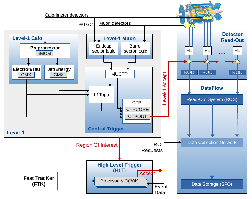
\includegraphics[width=.7\linewidth]{trigger_system}
    \caption{Schematic view of the ATLAS trigger and data acquisition system.}
    \label{fig:trigger_system}
\end{figure}
%%% Local Variables:
%%% mode: latex
%%% TeX-master: "../search_for_DM_LED_with_ATLAS"
%%% End:
